% !TEX program = xelatex
\documentclass[sigconf,nonacm,anonymous,review]{acmart}

\usepackage{kotex}
\usepackage{graphicx}
\usepackage{booktabs}
\usepackage{array}
\usepackage{enumitem}
\usepackage{balance}
\usepackage{amsmath}
\usepackage{amssymb}
\usepackage{newunicodechar}
\usepackage{dblfloatfix}
\setlist[itemize]{leftmargin=*,nosep}
\settopmatter{printacmref=false, printccs=false, printfolios=true}
\renewcommand\footnotetextcopyrightpermission[1]{}
\pagestyle{plain}

% ---- unicode symbols used in the Korean body (xelatex) ----
\newunicodechar{→}{\ensuremath{\rightarrow}}
\newunicodechar{↔}{\ensuremath{\leftrightarrow}}
\newunicodechar{≤}{\ensuremath{\le}}
\newunicodechar{≥}{\ensuremath{\ge}}
\newunicodechar{≈}{\ensuremath{\approx}}
\newunicodechar{×}{\ensuremath{\times}}
\newunicodechar{∈}{\ensuremath{\in}}
\newunicodechar{±}{\ensuremath{\pm}}
\newunicodechar{·}{\textperiodcentered}
\newunicodechar{°}{\textdegree}
\newunicodechar{τ}{\ensuremath{\tau}}
\newunicodechar{✓}{\ensuremath{\checkmark}}
\newunicodechar{✗}{\ensuremath{\times}}
\newunicodechar{⓪}{(0)}
\newunicodechar{①}{(1)}
\newunicodechar{②}{(2)}
\newunicodechar{③}{(3)}
\newunicodechar{④}{(4)}
\newunicodechar{⑤}{(5)}
\newunicodechar{⑥}{(6)}
\newunicodechar{⑦}{(7)}

% placeholder box for figures whose plots are deferred this round
\newcommand{\figtodo}[1]{\fbox{\parbox[c][2.6cm][c]{.92\linewidth}{\centering\itshape #1\\[3pt]\normalfont\footnotesize[\,placeholder: plot inserted once measurements are in\,]}}}

\title{OVLA: On-device Verification of LLM-Generated IoT Automations via Timeline IR}
\author{Anonymous Submission}
\affiliation{\institution{Submitted to SenSys 2027}\country{}}
\email{}

\begin{document}

\begin{abstract}
Smart home automation increasingly relies on Large Language Models (LLMs) to translate natural language (NL) user intents into executable reactive rules. However, deploying these rules directly on edge hubs poses severe reliability and safety risks since reactive IoT automations are temporally complex, involving precise triggers, durations, and repetitions. Existing validation methods rely heavily on human code inspection, offline experts, or resource-heavy cloud LLM re-checks, failing edge privacy and latency constraints. To tackle this challenge, we present OVLA, an on-device pipeline for deterministic, LLM-free verification of IoT automations before deployment. OVLA bridges the gap between informal natural language and strict execution using Timeline IR, a compact, machine-checkable representation of temporal behavior. The pipeline first translates the user's NL intent into a typed Timeline IR; the user confirms a deterministic plain-language rendering of this IR, which then serves as the reference specification of the intended behavior. OVLA then automatically synthesizes reference event traces and boundary cases from this IR. An efficient verifier simulates the generated rule code against these traces to detect behavioral discrepancies and guide automated repairs via counterexamples. Evaluated with a local, quantized ≤9B model across 382 automations, OVLA caught every faulty program in our evaluation set, repairing 31\% of them and rejecting the rest fail-closed; the only cost was two commands rejected because their gated-run lowerings never became valid within the repair budget. Under 1,562 injected temporal bugs, it detected 99.3\%, while its synthesized scenarios exercised 97.4\% of specification-side obligations and 96.8\% of generated-code branches, raising the share of correctly deployed automations from 90.8\% to 93.2\%, all without any LLM in the verification loop.
\end{abstract}

\keywords{IoT automation, LLM code generation, reactive-temporal code, deterministic verification, on-device, trace equivalence}

\maketitle

\section{Introduction}

IoT automation is rapidly moving toward LLM-based code generation. A user states the desired behavior in natural language, and an LLM turns it into a reactive rule the platform can execute. Yet the final step of this workflow, deciding \emph{whether the generated code is correct to deploy}, has no deterministic gate. The missing piece is a reference to check the code against; the natural-language request contains the intent, but not in a form that can serve as one.

\textbf{Why this is hard: there is nothing to check against.} The automations we target are \emph{reactive-temporal}: \emph{reactive} because their behavior is driven by events (triggers, waits on conditions), and \emph{temporal} because it is also driven by time (schedules, periodic execution, sustained durations such as ``if it persists for more than N minutes''). With timers, counters, and multi-step state, the behavior is defined over a timeline rather than at a single instant, and in our setting it is deployed as \emph{code}, not as a fixed rule template. Two properties make deciding their correctness hard. First, no oracle is given. The intended behavior is fixed by the user's request, but nothing provides it as a checkable artifact: the request was given moments ago, it may admit more than one valid realization, and no benchmark supplies a gold answer. Unlike text-to-SQL, whose benchmarks supply a gold denotation, or algorithmic code, which ships with input-output tests, a reactive automation's output is a future sequence of device actions that no external source labels as correct, so the reference has to be constructed rather than looked up. Second, the same intended behavior admits many syntactically different yet behaviorally equivalent realizations, so checking a generated program by matching it against any single reference text is neither sound nor complete. Deciding whether the code is correct therefore means reasoning about its behavior over time, not about its syntax or a single output.

\textbf{Running example.} Suppose a user requests ``whenever the temperature rises above 25°C, turn on the air conditioner.'' We read ``rises above'' as an edge-triggered intent: the AC should be switched on once per upward crossing, not continuously while it stays hot. Figure~\ref{fig:idiom} shows three lowerings, sketched in JoI, the automation DSL of our target platform (\S4). A detects the crossing by comparing the previous and current readings; B keeps a flag that is set on firing and reset when the temperature falls back. A and B share almost nothing syntactically yet behave identically, so no syntactic comparison can certify one against the other. C is the most natural-looking lowering because it reads like the request itself, and it is the wrong one: under periodic execution it re-fires on every tick while the temperature stays above the threshold. All three are syntactically valid and look plausible; only the action traces separate them, and because repeated On() commands leave the AC in the same visible state, the user may see nothing wrong. This is the failure mode we eliminate: \textbf{deployed code that silently diverges from what the system told the user it would do}. (In the sketches, \texttt{cron} sets when the script starts, \texttt{period} is the tick interval in milliseconds, and \texttt{code} is the body executed on every tick; \texttt{:=} initializes a persistent variable once, while \texttt{=} updates it per tick.)

\begin{figure*}[t]
\centering
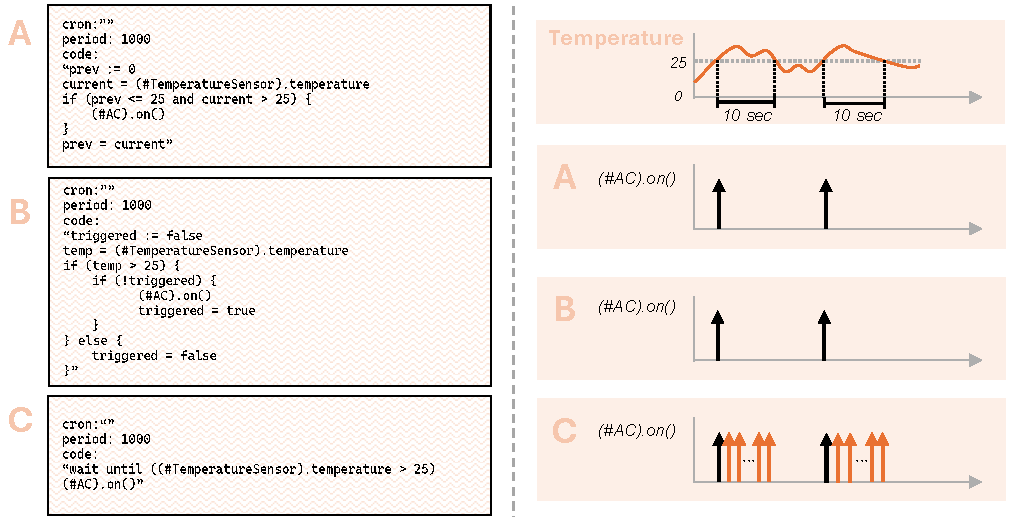
\includegraphics[width=\textwidth]{figs/trace.pdf}
\caption{Three lowering sketches of one intent (``whenever the temperature rises above 25°C, turn on the air conditioner'') and their action traces. A and B produce identical traces; C fires on every tick while the threshold is exceeded.}
\label{fig:idiom}
\end{figure*}

\textbf{Why existing checks do not close the gap.} Prior verification of automations targets fixed criteria, not intent. A large body of work checks hand-authored trigger-action rules: model checkers prove safety properties, inter-rule conflicts, or security (e.g., AutoTap~\cite{autotap}), and runtime monitors flag deviations from mined invariants~\cite{hawatcher}. This is by design, not omission. When the user writes the rule directly, the rule \emph{is} the intent, and the risks worth checking (conflicts, security) are defined without reference to any one task's intended behavior. When the user stops being the author, the question changes: once an LLM writes the code from a natural-language request, what the user said and what was produced become two separate artifacts that can disagree, and only then does intent-conformance become a question to check.

In that generation setting the gap is real but unfilled, and whether a system closes it turns on one question: does an oracle already exist? Generators of algorithmic IoT code can check their output against executable tests or labeled accuracy, much as text-to-SQL checks denotation, so conformance is a non-issue (e.g., GPIoT~\cite{gpiot}). Reactive automations have no such ready-made oracle, so natural-language-to-automation generators settle for weaker proxies: schema validity (the framework accepts the JSON), grounding feasibility, ground-truth command matching, or an LLM judge; and even those that show the generated rule back to the user have the user confirm it by hand rather than checking the code against it (AwareAuto~\cite{awareauto}). None checks deterministically that reactive-temporal code behaves as intended. The missing piece is not a better model but a reference to check against.

\textbf{Why not an LLM judge.} The one remaining option that targets intent directly is to ask another LLM whether the code matches the request. But an LLM judge is unstable as a deployment gate. A deployment decision is binary: two behaviorally identical programs must receive the same deploy/reject verdict. Yet we find that on behavior-preserving programs that differ only in idiom, an LLM judge's verdict flips even at temperature 0 (\S3). Larger models still flip, and cloud models violate the privacy and latency constraints of the edge. A gate whose verdict tracks the surface form of the code is not fit to gate deployment.

\textbf{OVLA.} We present OVLA. Its key idea is to \emph{derive the missing reference} at authoring time and then check against it deterministically. From the request OVLA builds a candidate Timeline IR; the user confirms its deterministic plain-language Rendering; and that confirmed IR becomes a per-automation behavioral oracle. The generated JoI code is then checked against the oracle by bounded trace-equivalence over the finite set of transition points the IR defines: both are run on events synthesized at those points (timer expirations, condition thresholds, cycle restarts), and their action traces are compared. The LLM is confined to \emph{generation}, proposing the IR and lowering it to code; both the rendering step and the equivalence check are deterministic and LLM-free, so a conformant automation can be deployed at once with no cloud-side review. \emph{Precisely because} lowering is an LLM stage, a deterministic checker is needed.

\textbf{Scope and assumptions.} OVLA's input is a natural-language command that names a specific reactive-temporal behavior. Inferring what behavior a user would want from an affective or underspecified goal (``make it cozy'') is a separate intent-elicitation problem (Sasha~\cite{sasha}, SAGE~\cite{sage}) and is out of scope; residual ambiguity in a specifiable command is surfaced by the deterministic Rendering and resolved at confirmation, not by the verifier. Confirming the IR is presented as a plain-language judgment rather than a programming task: the dimensions a user controls in reactive-temporal automation are limited and enumerable (start time, period, trigger and condition, action and its arguments, sustain and delay durations), Timeline IR expresses only these slots, and deterministic Rendering surfaces them verbatim as a timeline the user reads rather than code (\S8.3). Approving an IR is thus a closed judgment over the finite control slots the command named, not the authoring of an arbitrary formal property.

\textbf{Two-layer guarantee.} We are explicit about how far the guarantee reaches. \textbf{Layer A (NL→IR)}: the system captures intent as IR and presents it in plain language, but we do not measure non-expert confirmation success \emph{itself} in this round (no human-subjects study, \S9). \textbf{Layer B (IR→code)}: once the IR is approved, OVLA prevents the generated code from silently diverging from that displayed IR within a bounded behavior region. OVLA's guarantee lies in Layer B.

\textbf{Deployment setting.} We assume a home edge device rather than the cloud, for privacy (sensor data never leaves the home) and latency. This constraint excludes a cloud LLM judge from the gate, so the gate must be an LLM-free deterministic check. A single design decision yields both trust (no probabilistic judge) and deployability (milliseconds, no model call).

\medskip\noindent\textbf{Contributions.} To our knowledge, OVLA is the first system for LLM-generated reactive-temporal IoT automations to turn intent-conformance into a deterministic pre-deployment check, using a user-confirmed behavioral IR as the oracle rather than a probabilistic judge or manual review.
\begin{itemize}
\item \textbf{C1. Timeline IR.} A single representation plays two roles at once: (a) a surface that is deterministically rendered to plain language for the user to approve, and (b) a machine-checkable behavioral reference for checking reactive-temporal code. An approved NL sentence can serve only (a); a formal property only (b). A representation that is both is the contribution; since prior work already generates confirmable temporal IR, our claim is the \emph{combination} of deterministic LLM-free verification, rendering, and on-device operation (\S2).
\item \textbf{C2. Deterministic deployment gate.} IR→FSM→boundary event→bounded trace-equivalence performed without an LLM, fail-closed (pass=deploy / fail=repair or reject). When it flags, the flag is a real behavioral divergence under the defined observation model (rejection-sound).
\item \textbf{C3. On-device realization.} Generation uses a 4-bit quantized model of at most 9B parameters without fine-tuning, and the gate makes no LLM call at all, so verification runs in milliseconds without the cloud. The guarantee does not depend on the size or quality of the generation model.
\item \textbf{C4. Evaluation.} We demonstrate system safety (silent IR-code divergence 9.2\%→0, \S8.1), verifier detection (\S8.2), rendering faithfulness (\S8.3), and on-device cost and deployment (\S8.4) component by component.
\end{itemize}

\textbf{Focus of the contribution.} OVLA removes a failure mode that survives user approval: even when the approved IR is acceptable, reactive-temporal lowering can introduce state, timer, and boundary errors that make the deployed code diverge from it. OVLA is the deterministic on-device gate that catches exactly this.

\section{Related Work and Positioning}

\begin{table*}[t]
\centering
\caption{Positioning of work that checks generated automations.}
\label{tab:positioning}
\begin{tabular}{llll}
\toprule
System & Artifact checked & Verification reference & Verification method \\
\midrule
AutoTap & TAP rules & safety property & model checking \\
ChatIoT & HA automations & format/value & LLM judge \\
GPIoT & algorithmic code & external tests & test execution \\
AwareAuto & automation rules (JSON) & grounding feasibility & no behavioral check \\
LACE & access-control policy & intended behavior & probabilistic NLI \\
\textbf{OVLA} & \textbf{reactive-temporal code} & \textbf{user-confirmed IR behavior} & \textbf{deterministic trace (LLM-free)} \\
\bottomrule
\end{tabular}
\end{table*}

IoT automation is rapidly shifting toward LLM-based generation of executable rules from natural language, and attempts to check the generated artifacts have accumulated alongside adjacent work on rule verification and code generation. We group prior work by \emph{what it checks after generation}: since nearly all systems take natural language as input, the discriminator is the check, not the input.

\textbf{NL-to-automation generation.} A variety of LLM-based systems turn natural-language requests into executable automations. Sasha~\cite{sasha} interprets vague goals such as ``make it cozy'' conversationally and maps them to device settings, deciding actions on the spot with single-shot reasoning. SAGE~\cite{sage} builds tool-call sequences through a tree of LLM prompts, expresses persistent commands as a Python condition with a polling loop, and corrects itself from execution feedback at runtime. ChatIoT~\cite{chatiot} translates natural language into Home Assistant trigger-action automations with multiple LLM agents, and a separate ``Evaluator'' agent assesses format compliance and request satisfaction, correcting format and value mismatches. Giudici et al.~\cite{giudici2025} present a chatbot that takes home context and energy data and generates Home Assistant routines (JSON), judging correctness by whether the Home Assistant framework accepts the JSON. IoTGPT~\cite{iotgpt} produces SmartThings rules through decompose--derive--refine stages, catches API violations and runtime errors (but not intent mismatches) with LLM self-correction in a virtual SmartThings environment, and measures accuracy by matching ground-truth commands. AwareAuto~\cite{awareauto}, the most expressive in this line, builds a confirmable reactive-temporal rule with event/state modes, delays, branches, and sequencing from natural language, shows it to the user in a panel, and lowers it to executable JSON. \emph{Across this line, automatic checks stop at format adequacy, API validity, or device-grounding feasibility. Even in AwareAuto, intent consistency is evaluated by researcher annotation, and the user-facing confirmation text is generated prose rather than a deterministic rendering; none of these systems verifies that the generated code behaves as intended.}

\textbf{Verification and analysis of automations and commands.} A rich body of work verifies and analyzes hand-authored TAP rules with formal techniques. AutoTap~\cite{autotap} synthesizes or repairs TAP rules, modeled as transition systems, to satisfy LTL safety property templates chosen by the user. TAPInspector~\cite{tapinspector} extracts rules from market apps, builds a concurrent automaton that captures timing and scheduling, model-checks safety and liveness properties with NuSMV, and finds inter-rule interaction vulnerabilities; TAPFixer~\cite{tapfixer} detects vulnerabilities against negated safety and liveness properties and repairs them automatically. iRuler~\cite{iruler} recovers inter-rule information flows with NLP and finds inter-rule vulnerabilities with SMT and model checking, while Soteria~\cite{soteria} extracts state models from SmartThings apps and model-checks safety and security properties. AutoIoT~\cite{autoiot_maude} checks LLM-generated rules with Maude rewriting logic for four inter-rule conflict types, and HAWatcher~\cite{hawatcher} detects runtime anomalies against mined correlation invariants. DS-IA~\cite{dsia} checks the device-grounding feasibility of a command with a deterministic cascade and rejects fail-closed before execution, and TaskSense~\cite{tasksense} checks whether an LLM-generated sensor-coordination plan is solvable and respects tool dependencies, a structural well-formedness check rather than a behavioral one. AgentSpec~\cite{agentspec} enforces trigger-predicate safety rules on LLM agents at runtime with a deterministic DSL, but the rules are fixed and hand-written rather than derived from the request being served. The verification reference in this line is a fixed safety property, an inter-rule conflict, a security vulnerability, or feasibility, not the per-task intended behavior (HAWatcher operates post-deployment at runtime; DS-IA and TaskSense check feasibility and structure). Whether a single, especially generated, automation conforms to the user's intended behavior is not addressed. TAP rules do carry temporal behavior, including triggers, stays-for durations, and cron-style schedules, but there it is a platform \emph{primitive}: the author fills slots and the engine implements the mechanism. In reactive-temporal code such as JoI scripts, no primitive exists for edge detection, sustained conditions, or counting; the author, here an LLM, realizes the mechanism as an \emph{idiom} built from persistent variables, conditions, and per-tick execution. Slot errors are visible on the face of a rule; mechanism errors are silent, and they are exactly where lowering bugs live.

\textbf{Code generation with an existing oracle.} Some generation work verifies comparatively easily because an executable reference already exists for the target code. GPIoT~\cite{gpiot} generates signal-processing and ML algorithm code from natural-language requirements via specifications, using an on-device fine-tuned SLM, and verifies it with pass@k execution tests. AutoIOT~\cite{autoiot_mobicom} likewise generates runnable sensing/ML Python programs from natural language and verifies them with execution success rates and labeled accuracy. Outside IoT, text-to-SQL verifies against the denotation of a gold query~\cite{spider}, and CodeT~\cite{codet} and Self-Debug~\cite{selfdebug} verify generated code with unit tests. These checks are possible because the domain supplies an executable oracle, and reactive automation has none. OVLA derives that oracle from the approved IR; trace-equivalence is the counterpart of execution accuracy in this domain.

\textbf{Work that directly targets intent conformance.} Work that directly asks whether the generated artifact matches the user's intent is rare. LACE~\cite{lace} back-translates a generated static access-control policy into natural language with deterministic templates, judges semantic equivalence against the original request with a fine-tuned NLI model, and adds Z3 conflict detection and OPA re-validation. SimuHome~\cite{simuhome} is a benchmark that judges agent behavior against goal states in a time-accelerated simulator, scoring feasible tasks with deterministic simulator assertions and infeasible or ambiguous tasks with LLM-judge majority voting; it shows that 18 LLM agents largely fail to self-correct their own reactive-temporal errors (\S3). SimuHome is closest to us in checking behavior against a simulator goal state, but the goal is authored by the benchmark rather than approved by a user, it evaluates agents rather than gating deployment, and its artifact is a tool sequence rather than a reactive automation. \emph{LACE is closest in problem framing, but its target is a timeless static policy, its judgment is probabilistic NLI, and no user is in the loop, so its reported ``100\% correctness'' is self-certified by the model. Even where intent is addressed, the verdict rests on a probabilistic model and is unstable as a deployment gate.}

\textbf{Positioning.} The two nearest neighbors are LACE and AwareAuto. LACE checks intent equivalence, but on static policies, probabilistically, and without a user. AwareAuto builds a confirmable reactive-temporal representation, but does not verify behavior. OVLA starts where both stop: it takes the user-approved IR as the behavioral reference and checks the generated reactive-temporal code with deterministic, LLM-free trace-equivalence, before deployment, on-device. Combining generation with verification is standard in this field and is not our claimed novelty (Table~\ref{tab:positioning}); the novelty lies in user-approved deterministic behavioral verification and the multi-role IR. In the table, the \emph{artifact} column states what each system checks, in that system's own terms; the \emph{verification reference} states what the artifact is checked against; and the \emph{verification method} states how. What makes OVLA unique is not any single cell but the \emph{row combination}: checking generated reactive-temporal code against the user-confirmed IR behavior with a deterministic, LLM-free trace.

\section{Problem and Motivation}

Together, \S1 and \S2 leave a clear task: a gate is needed that decides, before deployment, whether LLM-generated reactive-temporal code behaves as the user said. This section first establishes the requirements such a gate must meet in our setting, then weighs each candidate checking approach against them, and finally measures the one remaining candidate, an LLM judge, ourselves.

\textbf{Three requirements for a deployment gate.} \textbf{R1 (reference).} No reference is given. The intended behavior is fixed by the user's request, which arrived moments ago, but nothing provides it as a checkable artifact. Algorithmic code carries an executable oracle in the form of input-output pairs and is checked by running tests (GPIoT~\cite{gpiot}, \S2); for reactive-temporal code, the ``right output'' is a future sequence of device actions that no external source labels. The reference must be constructed, not looked up. \textbf{R2 (stability).} A deployment decision is binary: two programs with the same behavior must receive the same deploy/reject verdict. A checker whose verdict wavers under behavior-preserving rewrites is unfit as a gate, regardless of the quality of its individual judgments. \textbf{R3 (on-device).} Sensor data must not leave the home (privacy) and the verdict must be immediate (latency), so the gate must run on the edge without a cloud round-trip.

\textbf{Candidate 1: syntactic or structural comparison.} The simplest check is to match the generated code against some reference text. But as the temperature example of \S1 (Figure~\ref{fig:idiom}) shows, the same intent is realized by syntactically unrelated idioms (a prev/curr comparison vs.\ a triggered flag), while the bug (wait-until) is the one that most resembles the request. Near-miss bugs one tick or one comparison away look identical to valid variants. Syntactic or structural matching can neither certify valid variants against each other nor catch the bug, so it is neither sound nor complete. Equivalence must be decided on behavior, not on syntax.

\textbf{Candidate 2: self-checking by the generating model.} One could ask the model that produced the code to inspect and repair it. SimuHome~\cite{simuhome} evaluated this path with 18 models: self-correction recovery was 8.0\% on time-based errors, 18.5\% on event-based errors, and 0.0\% on coordinated scheduling, and stayed at or below 67\% even with an oracle provided. The authors conclude that agents fail to detect their own faulty plans. A post-hoc self-check entrusted to the same stochastic process that generated the code is not a gate.

\textbf{Candidate 3: human inspection of the code.} One could show the generated code to the user for approval. But in TAP-Debug~\cite{tapdebug}, non-experts misread even the IF (event) and WHILE (state) of raw rules: misreadings occurred in 21 of 50 control-condition sessions, and all 21 failed the task. If this happens with a two-slot TAP rule, expecting users to inspect reactive-temporal code that realizes its mechanism through persistent variables and per-tick execution is untenable. What is shown to the user must be readable rather than code; this also motivates the deterministic Rendering of \S5.

\textbf{The remaining candidate: an LLM judge.} What remains is to hand the request and the code to a separate LLM and ask whether they match. This is plausible on its face and used in practice (ChatIoT's Evaluator, \S2), and existing results do not rule it out. We therefore measure whether this candidate meets R2 (OVLA's IR and verifier play no part in this experiment). We presented programs with exactly identical behavior (trace-exact) that differ only in idiom, and measured how often the judge's accept/reject verdict flips. Even in the deterministic setting at temperature 0, a 9B model flipped on 27\% of pairs and a strong cloud model on 10.6\%. The rewrite types divide into surface rewrites (SEL = selector order, AND = $A{\wedge}B{\leftrightarrow}B{\wedge}A$, VAR = variable renaming) and logic/arithmetic rewrites (ADD = $x{+}n{\leftrightarrow}n{+}x$, BR = branch swap, DN = double negation, DM = De Morgan, IDM = idiom replacement) (Figure~\ref{fig:instability}). Purely surface rewrites already flip up to 9\% of the 9B judge's verdicts (14\% for the cloud judge), and logic and arithmetic rewrites flip up to 81\%. No ground-truth label is needed: the flip itself evidences instability. The point is not the miss rate; on cleanly injected bugs, strong models are in fact competent detectors. The point is that \emph{any} probabilistic judge yields an unstable deployment policy under behavior-preserving rewrites. The instability persists with larger models, and majority voting does not push it below the temperature-0 baseline, because voting cancels sampling noise but not the systematic dependence on surface form (Table~\ref{tab:instab}). This violates R2, and the last candidate falls. OVLA's verdict, by contrast, depends only on behavior over a bounded set of traces, so under the same rewrites its flip rate is 0 by construction.

\begin{figure}[t]
\centering
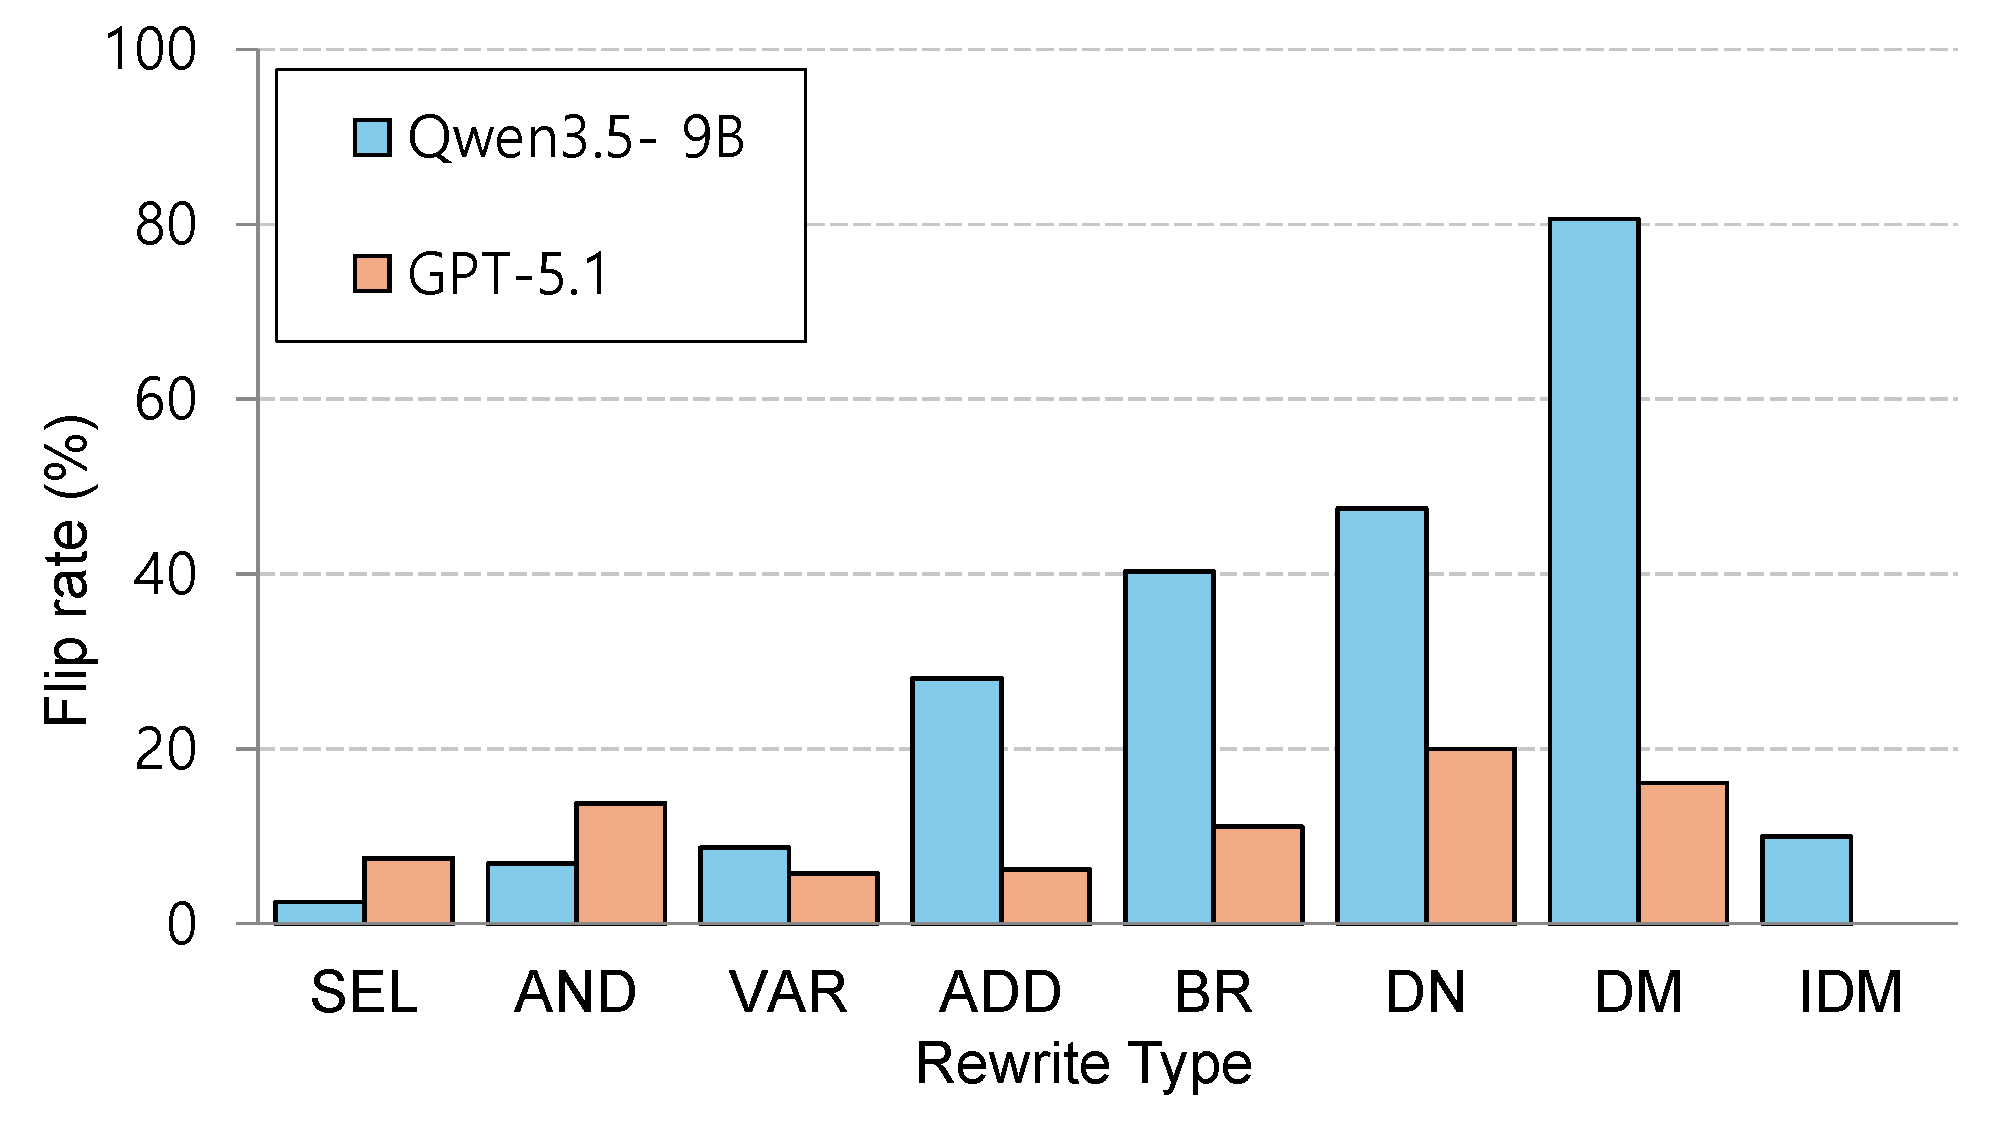
\includegraphics[width=\linewidth]{figs/instability.pdf}
\caption{LLM judge verdict flip rate by rewrite type on behavior-identical programs (temperature 0).}
\label{fig:instability}
\end{figure}

\begin{table}[t]
\centering
\caption{Overall flip rate by judge configuration; OVLA's trace check flips on none of the same rewrites.}
\label{tab:instab}
\begin{tabular}{lcc}
\toprule
Judge configuration & 9B & GPT-5.1 \\
\midrule
deterministic (temp=0) & 27.0\% & 10.6\% \\
+ sampling (temp=0.7) & 34.4\% & 12.8\% \\
+ majority vote (K=5) & 31.2\% & 13.5\% \\
\textbf{OVLA (deterministic trace)} & \textbf{0\%} & \textbf{0\%} \\
\bottomrule
\end{tabular}
\end{table}

\textbf{The surviving design.} With every candidate eliminated, rereading the requirements reveals the shape of the answer. By R1, the reference must be \emph{derived} from intent the user has confirmed; by R2, the check must be deterministic over behavior (traces), not syntax; by R3, it must run lightweight, with no LLM call. The artifact that satisfies all three at once is the Timeline IR (\S5), and the deterministic trace-equivalence check over it is the verifier (\S6). (The judge in this motivating experiment compares NL against code; it is a different experiment from the judge of \S8.2, which is given the IR and compares it against code.)

\section{System Overview}

\textbf{Target platform.} OVLA runs on the edge hub of a commercial IoT platform whose execution DSL is JoI. A JoI script consists of a start time (\texttt{cron}), a tick interval (\texttt{period}), and a body executed on every tick (\texttt{code}); it is reactive-temporal code that implements its behavior directly with persistent variables and conditions (\S1's sketches). This DSL is the target of lowering.

OVLA is organized around a single principle: the LLM is used for \emph{generation} (proposing the IR and lowering it to JoI), while the feasibility gate, the Rendering shown for approval, and the verifier are deterministic and make no LLM call. Figure~\ref{fig:arch} shows the full pipeline, read in two phases.

\textbf{Phase 1: Generation (on-device LLM).} ① Semantic parsing (intent analysis, device mapping, tool mapping) processes the user's NL command. ② From its output a \textbf{Timeline IR} is extracted; the \textbf{feasibility gate \texttt{IR∈L(G)}} deterministically rejects structurally impossible IRs, and the surviving IR is turned into plain language by the deterministic \textbf{Rendering}. ③ The rendered text is shown to the user, and ④ on confirmation the Timeline IR is fixed as the reference. ⑤ The confirmed IR is \textbf{lowered} to JoI code.

\textbf{Phase 2: Verification (deterministic, LLM-free).} ⑥ The verifier checks the generated JoI. The confirmed Timeline IR enters as the behavioral reference (the reference arrow in Figure~\ref{fig:arch}); after the \textbf{L1} static check (well-formedness of the generated JoI), an FSM is derived from the IR, boundary \textbf{events are synthesized}, and the IR simulator and the JoI simulator are run on the same events to compare \textbf{trace-equivalence}. ⑦ The verdict is one of two: deploy on pass, or \textbf{reject (fail-closed)} when repair is exhausted. On a mismatch, control returns to lowering (⑤) with a \textbf{counterexample} and only the JoI is regenerated (dashed arrow; the IR is the approved reference and stays fixed).

\begin{figure*}[t]
\centering

\includegraphics[width=\textwidth]{figs/system.pdf}
\caption{OVLA system overview. ①{--}⑤ generation, ⑥{--}⑦ verification; the dashed arrow is the counterexample-guided repair loop.}
\label{fig:arch}
\end{figure*}

\textbf{Three checks, three places.} The three checks sit at different points on different artifacts. \textbf{Feasibility = \texttt{IR∈L(G)}} is a structural gate on the \emph{IR} as a typed tree, right after IR extraction and before lowering. \textbf{L1} is a static well-formedness check on the \emph{generated JoI code}, after lowering and before L2. \textbf{L2} is \emph{behavioral trace-equivalence}. We do not collapse the three into one stage: L2 is the core, and feasibility and L1 are the gates that support it.

\textbf{Roles of the IR.} A single Timeline IR plays four roles: the artifact the user approves (its plain-language surface), the verification reference, a generation scaffold, and a structural signature. The upstream semantic parsing (intent analysis, device/tool mapping) is substrate and not a contribution of this paper. (Device mapping runs in parallel with IR extraction but is drawn sequentially in the figure.)

\section{Timeline IR}

Timeline IR is designed to hold two properties at once. First, it is rendered to plain language deterministically (without an LLM) so the user can approve it. Second, it is a machine-checkable behavioral reference. NL→IR is an LLM stage, but IR→Rendering is deterministic, so the text the user sees reflects the IR exactly, with no room for hallucination: what is displayed is what is checked.

\textbf{Closed control dimensions and primitive ops.} Both properties follow from how the IR represents behavior. The dimensions a reactive-temporal command controls are closed and enumerable: start and schedule (\texttt{start\_at}), period (\texttt{cycle.period}), triggers and conditions (\texttt{wait}'s cond and edge, \texttt{if}'s cond), actions and their arguments (\texttt{call}), sustain and delay (\texttt{wait.for}, \texttt{delay}), and state and counting (persistent variables, \texttt{cycle.count}, \texttt{break}). Timeline IR assigns one primitive op to each dimension, encoding exactly what the command specified, no more and no less, directly on a timeline. This canonical, minimal, complete form yields both properties at once. (a) The deterministic Rendering puts these slots into plain language without adding information, so approving an IR is a closed judgment over the finite slots the command named, not the authoring of an arbitrary formal property. (b) The same representation doubles as a machine-checkable behavioral reference with nothing omitted. The closed op set is exactly what the grammar G below ranges over.

\textbf{Finite-state view.} The IR views reactive behavior as a finite set of obligations: no recursion, no unbounded loops, only bounded timers, counters, and finite control. This is not a model-checking target but a view that makes the objects of checking enumerable (it is not a timed automaton).

\textbf{Typed tree and dependency grammar G.} The IR is a typed tree, and a dependency grammar G fixes which structures are legal: exactly one \texttt{start\_at} (and at most one top-level cron), no \texttt{cycle} inside \texttt{cycle.body} (no nesting), \texttt{then}/\texttt{else} only as children of \texttt{if}, \texttt{break} only inside a \texttt{cycle}, and \texttt{cycle} requires a period (\texttt{until} is optional; absent, the cycle repeats within the bounded horizon). Membership \texttt{IR∈L(G)} is deterministically decidable. The same single pass over the typed tree also yields the IR's structural class τ(IR), the combination of G productions the IR instantiates, which \S7 uses to route lowering exemplars.

\textbf{Feasibility gate.} This membership test is the first gate in the pipeline. Right after IR extraction, before lowering and any code-level check, it deterministically decides whether the IR belongs to G and rejects structurally impossible IRs (nested cycles, double cron, misplaced then/else, break outside a cycle). Its correctness holds by construction (grammar membership) and needs no experiment. The guarantee, however, rests on the assumption that the extractor \emph{transcribes} the user's words literally: if the LLM silently flattens an illegal structure, a valid IR passes G with the wrong meaning, leaving a residue for confirmation to catch. The extractor is therefore designed to transcribe, not to correct.

The operators are \texttt{start\_at}, \texttt{wait} (cond, edge, for), \texttt{delay} (duration), \texttt{read}, \texttt{call}, \texttt{if} (then/else), \texttt{cycle} (period, count, until, body), and \texttt{break}. Figure~\ref{fig:ir} shows two examples. (a) is the temperature example of \S1: ``whenever the temperature rises above 25°C'' is encoded as \texttt{wait(Temperature > 25, edge: rising)} inside a \texttt{cycle}, and the Rendering surfaces the \texttt{edge: rising} slot as ``each new occurrence'' and the \texttt{call} as ``Turn on the air conditioner.'' (b) is a schedule-driven automation: the \texttt{start\_at} cron becomes ``Start at 9:00 PM every day,'' \texttt{cycle.period} becomes ``Every 10 minutes,'' and the \texttt{if}-\texttt{call}-\texttt{delay}-\texttt{call} sequence becomes one conditional behavior sentence. Note that even the empty \texttt{else} branch is surfaced as ``Otherwise, do nothing.'': the Rendering neither drops nor adds slots (\S8.3).

\begin{figure*}[t]
\centering
\begin{minipage}[t]{0.42\textwidth}
\centering
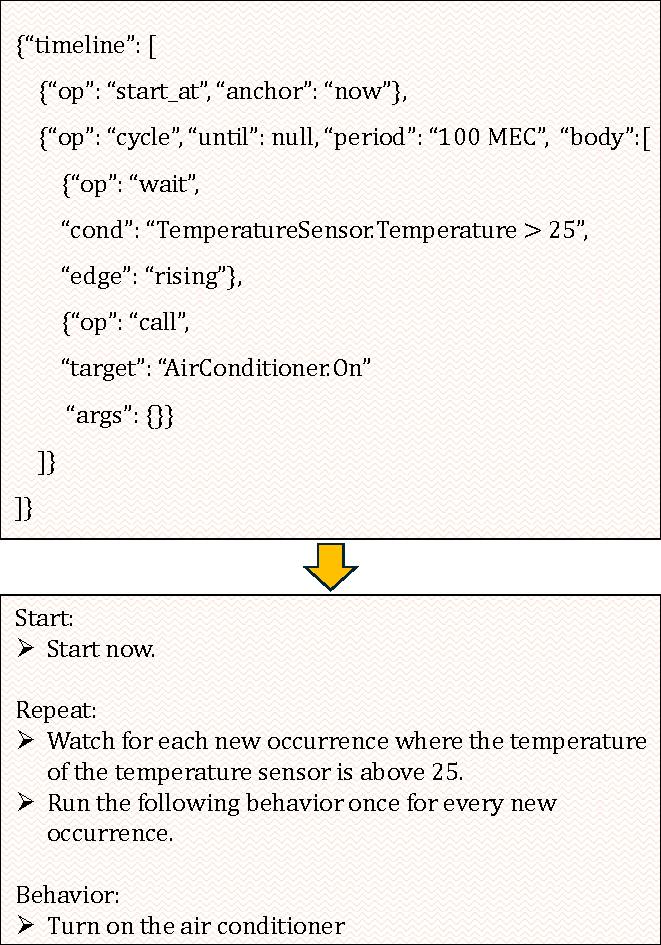
\includegraphics[width=\linewidth]{figs/Rendering1.pdf}\par
\small (a) Recurring edge trigger
\end{minipage}\hspace{0.04\textwidth}%
\begin{minipage}[t]{0.42\textwidth}
\centering
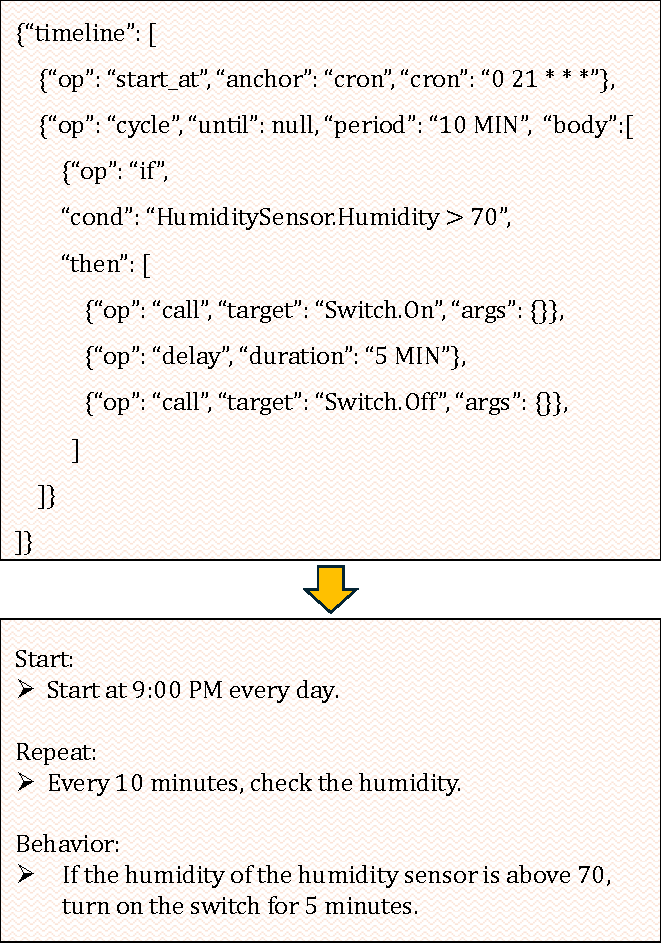
\includegraphics[width=\linewidth]{figs/Rendering2.pdf}\par
\small (b) Scheduled periodic check with branch and delay
\end{minipage}
\caption{Two Timeline IRs and their deterministic plain-language Renderings.}
\label{fig:ir}
\end{figure*}

\section{Verifier}

\subsection{Observation Model: Transition-Boundary Conformance}

The gate decides one thing: does the generated JoI code \emph{behave the same} as the approved IR? As \S2 observed, the execution DSL has no primitives for the IR's control dimensions, so the LLM realizes each IR behavior as an idiom: ``sustained for N minutes'' becomes a counter incremented on each poll tick that fires at a threshold; ``edge (whenever)'' becomes a triggered flag set on firing and reset when the condition clears (or a prev/curr comparison); ``every N minutes'' becomes periodic re-execution of the body. One IR behavior thus appears as several valid idioms and as countless near-misses one tick or one comparison off (Figure~\ref{fig:idiom}), and this idiom-realization point is exactly where bugs enter. Equivalence must therefore be decided on behavior (traces), not on syntax.

Deciding on behavior is tractable because reactive-temporal behavior has a formal skeleton: it is piecewise-constant over a finite abstraction of (time landmarks × sensor-value intervals × edges × bounded internal state). The only candidates at which behavior can change are guard thresholds, condition edges, time landmarks (delay, duration, period, cron), and state transitions. Because the IR admits only bounded control, with no recursion or unbounded loops, and fixes a 7-day horizon, this combination is finite, and one representative input per cell checks the entire cell. We take this as the observation model, \textbf{transition-boundary conformance}: two programs behave the same if their action traces agree, within a tolerance, at the boundaries where behavior can change (threshold crossings, condition edges, timer expirations, next-cycle restarts), over a fixed bounded horizon. This is an equivalence judgment focused on boundaries, not an equivalence proof over the whole input space, and it is what lets us run \textbf{bounded trace-equivalence} deterministically, solver-free, on-device, without full equivalence checking, model checking, or SMT. It is a deployment-time filter, not a replacement for heavyweight formal methods. (The internal-state axis cannot be dropped: hysteresis, toggles, counters, and sustains are not explained by sensor values alone.)

\subsection{Boundary Event Synthesis (IR-FSM → events)}

The core technique derives an FSM from the IR deterministically (no LLM) and synthesizes representative events at the IR's decision points. \texttt{call}/\texttt{wait}/\texttt{delay}/\texttt{read}/\texttt{if}/\texttt{cycle}/\texttt{break} become obligations; after-edges impose order, branches contribute guards, and \texttt{cycle} adds the obligation to re-arm for the next round. Around each boundary (guard threshold, edge, timer, cron, state transition) one representative event with a sustained boundary value is planted. The \emph{magnitude} of a crossing is irrelevant (31°C and 100°C fall in the same interval); what matters is timing. The synthesis is IR-based, not surface-syntax-based: it tracks read→sensor flows, handles abs/min/max with clamping, seeds both ends of a value domain (≥2 points to detect affine divergence), skips read-modify-write accumulators, and covers second edges where a condition clears and then holds again. The same synthesized event set is fed to the IR simulator and the JoI simulator, so the comparison is apples-to-apples.

\subsection{Trace-Equivalence and Omission Detection}

The IR simulator and the JoI simulator are run on the same events; the resulting action traces are grouped and deduplicated within a ±tolerance window (max 500ms, 10\%) and compared order-preserving. This comparison catches commission (actions that must not happen) and omission (required actions that are missing) at once, because \emph{silence} is part of a trace: an empty interval in the IR trace is an oracle saying ``nothing happens here.'' This works because the IR carries complete behavior; partial properties or LTL formulas do not pin down silence and so cannot catch omissions. For example, code that mistranslates ``check every 15 minutes'' into immediate reaction diverges from the IR in firing rate and timing on the IR's sustained-boundary scenarios (IR sparse or silent, JoI over-firing) and is flagged.

\subsection{What the Verdict Guarantees}

The verdict is deterministic and LLM-free. \textbf{T1 (determinism)}: the same (IR, code) pair always yields the same verdict. \textbf{T2 (rejection-soundness)}: when the checker flags, the flag is a real behavioral divergence under the defined observation model. We do not claim ``pass ⇒ correct.'' The trusted computing base is the two simulators, the tolerance, and the equivalence relation; the LLM is excluded. Soundness is supported by reduction to simulator fidelity rather than by proof, and the adequacy of the check is established empirically with exhaustive construct-derived mutation and two-sided coverage (\S8.2). Surviving mutants are characterized exhaustively rather than lumped into buckets.

\subsection{Limits of the Check}

For continuous arithmetic (action arguments that are continuous functions of a sensor), two or more representative points catch affine divergence, but arbitrary higher-order divergence is not covered; SMT is future work. Nothing beyond the bounded 7-day horizon is checked. A bug that matches the IR on all sustained inputs and differs only on transient glitches could in principle escape an IR-only check, but such a bug is self-contradictory and does not arise in practice. Variable-to-variable arithmetic without a threshold (e.g., \texttt{notify(\$t1-\$t2)}) offers no boundary to target, so only generic seeds apply: sign and structure bugs are caught, but value-specific bugs that fire only under particular value relations can be missed. This is a coverage limit, not a false-pass (soundness) issue: both simulators share the same values, so no false pass is created.

\section{Implementation}

OVLA uses a 4-bit quantized model of at most 9B parameters, without fine-tuning, on-device; generation is decomposed into stages (intent analysis / device and tool mapping / IR extraction / lowering). (Where GPIoT fine-tunes a 13B SLM and TaskSense relies on the cloud, we add a deterministic verifier to an off-the-shelf ≤9B model.)

\textbf{No-cloud co-design.} The no-cloud assumption excludes a cloud LLM judge from the gate, so the gate must be a deterministic, LLM-free check; the instability results of \S3 show that the same constraint-driven choice is independently justified.

\textbf{Structure-based exemplar routing.} The lowering prompt is assembled by routing on the IR's structural class. Every (IR, JoI) pair that passes the verifier is appended to an off-prompt exemplar bank and indexed by the deterministic structural signature τ(IR) computed during the feasibility pass (\S5): the combination of grammar productions the IR instantiates, such as cron-started cycle with sustain, or one-shot branch with delay. The signature is a construct-combination fingerprint, so classification needs no embeddings and no labels, and the same signature function serves both insertion and retrieval. At lowering time, the prompt injects only the best-K exemplars from the bucket matching the new IR's signature.

This design decouples the bank from the prompt: the bank grows as verifier-passed automations accumulate, while the prompt stays at a fixed K exemplars, and because a bucket's exemplars are stable, the assembled prefix is cache-friendly. Exemplars enter the bank only through the verifier, so a pair that once failed and was repaired contributes its corrected lowering for future requests of the same structural class. Routing acts only on the generator's prompt construction; the accept/reject verdict remains the deterministic, LLM-free check of \S6.

The IR is what makes this routing well-posed. Routing on the NL request would require embeddings and a similarity threshold; routing on the JoI code is unstable because the code is non-canonical (\S6.1); and certifying an exemplar as correct requires exactly the behavioral reference the IR provides. Removing the IR collapses the mechanism to generic retrieval over unchecked examples. We do not measure the effect of routing with an ablation in this round, so we describe the mechanism without quantitative claims about generation improvement.

\section{Evaluation}

The goal of the evaluation is not an accuracy contest but to establish, component by component, that each link of the workflow holds. The central result is system safety: silent IR-code divergence drops to zero (\S8.1).

\textbf{Setup.} \emph{Hardware}: the primary edge device is a Mac Mini M4 16GB (MLX 4-bit); an RTX 5090 (AWQ) serves as the reference for establishing accuracy. Safety results are backend-independent (on-device cost is measured on the M4, yields per backend; zero silent divergence is invariant). \emph{Dataset}: 382 automations in 24 categories. The commands were written to cover the reactive idiom families (triggers, edges, sustains, periodics, sequences, branches, counting) over devices the platform's service catalog supports, not curated to fit OVLA's grammar, and the ground-truth IRs passed an independent value-level audit that fixed the set at 382. \emph{Baseline}: the main comparison is the verification alternative, an LLM judge; for every judge we state, with the result it accompanies, the input artifact (request, IR, or code), temperature, and voting configuration. \emph{Metrics}: safety (silently divergent code deployed), detection (detection/FP/FN), faithfulness (surface rate), and on-device cost (latency distribution, memory, power).

\subsection{RQ1: System Safety}

Does OVLA prevent deployed code from silently diverging from the \emph{displayed IR}? Without the gate, 35 of 382 automations (9.2\%) would deploy while silently diverging from the IR displayed for approval. OVLA's bounded IR↔code check reduces this to zero: of the 35, 11 are repaired and 24 are rejected fail-closed; 2 further commands are rejected, for 26 rejections in total. The 2 further rejections are not verifier false positives: in both, every gated-run regeneration contained a real syntax or catalog violation within the 2-attempt repair budget, while the ungated run's independent generation of the same command happened to be correct. The cost is generation variance, 2 of 347 commands with a correct ungated lowering (0.6\%), not a misjudged program. The fraction of deployed automations that are correct rises from 90.84\% to 93.19\%. These numbers concern divergence from the \emph{displayed} IR (the confirmed-IR assumption), not whether the IR matched the user's true intent (Layer A; \S9).

\emph{Repair is not the safety evidence.} The safety claim lies in fail-closed: divergent code is repaired or rejected, and never deployed. Because the gate is deterministic, this property does not depend on generation stochasticity: whichever candidates the model produces, a divergent one cannot deploy silently. We report the repair-loop accounting (attempts, success rate, added latency, cases where repair broke correct code) and the 2 generation-variance rejections alongside. The hard core of rejects concentrates in sustain timing, read-modify-write, and multi-step automations, showing that fail-closed is not ``rejecting everything hard.''

\subsection{RQ2: Verifier Detection}

Does the verifier catch wrong code? We look at two layers, real bugs and synthetic bugs. The real layer comes from the 382-automation pipeline of \S8.1: all 35 real LLM lowering outputs that diverged from the displayed IR were flagged, and none escaped silently (the same 35 cases as \S8.1, restated here as detection rather than additional evidence).

\textbf{Mutation (stress coverage).} We then stress the mechanism with exhaustive construct-derived mutation (Table~\ref{tab:mutation}). Twelve operators generate every first-order mutant at every applicable site (331 seeds, 1,673 generated, 111 equivalents excluded against all scenarios), and 1,551 of 1,562 genuine mutants are caught (99.3\%). The adequacy of the synthesized scenario suite is measured as two-sided coverage (Table~\ref{tab:coverage}): the spec side exercises 97.4\% of IR-FSM obligations (342/351), with all 9 uncovered ones being unsynthesizable else-branch guards (7 variable-to-variable comparisons, 2 arithmetic); the implementation side exercises 96.8\% of generated-JoI branches (670/692). The 11 survivors are characterized exhaustively rather than bucketed: 8 are \texttt{>=}→\texttt{>} comparator mutants on sustain tick-counters whose 1-tick difference lies below the tolerance (max 500ms, 10\%; by design); 1 is a dropped duplicate call in a two-room fan-out (\texttt{call\_drop}); and 2 sit in a single arithmetic read-modify-write automation that boundary seeding cannot reach (one \texttt{call\_drop}, one \texttt{cmp\_direction}), the continuous-arithmetic limit of \S6.5. We separate three claims: ① it catches real lowering bugs (35/35, \S8.1); ② a one-construct perturbation of correct code is caught (the mutation kill rate); ③ silent mismatches in the 382 pipeline are zero (\S8.1). The mutation operators are not hand-picked: they are derived from the IR constructs, and every construct is reached by at least one operator. Mutation alone, being keyed to the same construct set the verifier checks, measures the reach of the mechanism rather than external validity; external validity rests on the real-fault layer above, and the implementation-side coverage shows the synthesized scenarios exercise the generated code, not only the spec. The soundness statement is rejection-sound, bounded-incomplete, and auditable (not ``pass ⇒ correct'').

\begin{table}[t]
\centering
\caption{Construct-derived mutation results (331 seeds, 12 operators).}
\label{tab:mutation}
\small
\setlength{\tabcolsep}{4.5pt}
\begin{tabular}{lrrrr}
\toprule
Operator & Gen. & Equiv. & Genuine & Caught (\%) \\
\midrule
arg\_numeric    & 146 & 1  & 145 & 145 (100) \\
enum\_flip      & 111 & 3  & 108 & 108 (100) \\
call\_drop      & 439 & 5  & 434 & 432 (99.5) \\
call\_add       & 202 & 4  & 198 & 198 (100) \\
tick\_scale     & 57  & 0  & 57  & 57 (100) \\
guard\_polarity & 197 & 0  & 197 & 197 (100) \\
comparator      & 163 & 38 & 125 & 117 (93.6) \\
assign\_init    & 71  & 13 & 58  & 58 (100) \\
cmp\_direction  & 163 & 31 & 132 & 131 (99.2) \\
arith\_op       & 42  & 12 & 30  & 30 (100) \\
break\_drop     & 28  & 4  & 24  & 24 (100) \\
wait\_drop      & 54  & 0  & 54  & 54 (100) \\
\midrule
Total           & 1,673 & 111 & 1,562 & 1,551 (99.3) \\
\bottomrule
\end{tabular}
\end{table}

\begin{table}[t]
\centering
\caption{Two-sided coverage of the scenario suite (spec: IR-FSM obligations; impl: generated JoI branches).}
\label{tab:coverage}
\small
\begin{tabular}{lrrr}
\toprule
Obligation & Total & Covered & (\%) \\
\midrule
\texttt{if}: then branch            & 166 & 166 & 100 \\
\texttt{if}: else branch            & 37  & 28  & 75.7 \\
\texttt{wait} (edge/sustain/re-arm) & 122 & 122 & 100 \\
arithmetic expr boundary (lo/hi)    & 26  & 26  & 100 \\
\midrule
Spec total (IR-FSM)                 & 351 & 342 & 97.4 \\
Impl: generated JoI branches        & 692 & 670 & 96.8 \\
\bottomrule
\end{tabular}
\end{table}

\textbf{vs.\ an LLM judge.} We compare the same IR↔code judgment against an LLM judge in the cloud-judge style of ChatIoT's Evaluator~\cite{chatiot}. The judge is given the IR, the JoI grammar, and the same equivalence definition including the timing tolerance, at temperature 0 with a single query; ground truth is objective (a verifier-clean lowering is correct, a non-trace-equivalent mutant of it is wrong). On 346 such programs (277 faulty, 69 correct), the 9B judge misses 36 of the faulty programs (recall 0.87) and falsely rejects 17 of the 69 correct ones; a strong cloud judge (GPT-5.1) still misses 16 (recall 0.94) and falsely rejects 14. On 30 behaviorally-correct idiom variants of the same intents (multi-GT), the 9B judge over-rejects 2 and the cloud judge 1, while the trace check passes all 30 idiom-invariantly. (This setting gives the judge the IR; it is a different experiment from the NO-IR motivating experiment of \S3.)

\subsection{RQ3: Rendering Faithfulness}

RQ3 checks one narrow prerequisite: \emph{does the deterministic Rendering expose every behavior-relevant IR difference in plain language?} We do not evaluate whether users approve the right IR (no human-subjects study; Layer A is \S9). We evaluate whether the approval surface is faithful, that is, whether the IR fields the gate consumes show up in the displayed behavior.

The claim is precise: the renderer exposes the IR fields that the checker and the lowerer consume, so faults in the IR-to-code relation are visible in the displayed behavior, and every behavioral difference in our test set produced a different Rendering. All 1,504 synthetic pairs across 8 fault classes surfaced as distinct text, with zero blind spots (Table~\ref{tab:faithful}). Of 57 real logic faults, 56 surfaced; the remaining one (C16\_5) is an upstream extraction defect in which the extractor leaked selector syntax into the IR, not a rendering blind spot. One pair suffices to show what surfacing looks like. In the oneshot↔wait-until class, the correct IR renders as ``If the charging state of the charger is fullyCharged, turn off the selected switch.'' while the faulty IR renders as ``Wait until the charging state of the charger is fullyCharged is true. Turn off the selected switch.'' A one-sentence difference exposes, in plain language, the same class of behavioral difference as the wait-until bug of \S1 (Figure~\ref{fig:idiom} C).

\begin{table}[t]
\centering
\caption{Rendering faithfulness: do behaviorally different IR pairs render differently?}
\label{tab:faithful}
\small
\begin{tabular}{lrrr}
\toprule
Fault class & n & Surfaced & Blind \\
\midrule
comparator                & 267 & 267 & 0 \\
polarity                  & 85  & 85  & 0 \\
wrong arg value           & 235 & 235 & 0 \\
wrong device              & 382 & 382 & 0 \\
timing/duration           & 74  & 74  & 0 \\
oneshot↔wait-until        & 150 & 150 & 0 \\
single↔cycle (whenever)   & 273 & 273 & 0 \\
AND-conjunct drop         & 38  & 38  & 0 \\
\midrule
Synthetic total (Part B)   & 1,504 & 1,504 & 0 \\
Real logic faults (Part A) & 57  & 56  & 1 \\
\bottomrule
\end{tabular}
\end{table}

\textbf{What does not surface.} This result does not mean every kind of error shows up in the text. (a) Device-name ambiguity: the same text can be interpreted onto different device bindings; binding is handled by the parallel precision channel. (b) Misread domain terms: a user may read the text differently, which is human behavior we do not evaluate. (c) Missing intent: what the user never said is absent from the IR and hence from the Rendering. (d) Unsupported constructs rejected before rendering. Our claim is that reactive-temporal \emph{logic} faults surface in plain language, something prior work shows is hard even to read off raw rules (TAP-Debug~\cite{tapdebug}: all 21 misreadings led to task failure).

\subsection{RQ4: On-Device Cost and Deployment}

\textbf{On-device cost.} We report latency as a distribution (p50/p95/worst) rather than a mean, together with peak memory, power, repair counts, and the \emph{worst-case verifier runtime by complexity} (by the number of triggers, timers, state variables, quantifiers, devices, and boundary events, not LOC). The key figure is the verification-cost comparison (Figure~\ref{fig:rq4}(a)): the LLM-free verifier costs milliseconds and \$0, a local 9B judge costs seconds and VRAM, and a cloud judge costs seconds plus fees plus a network dependency. We also report the unsupported-intent rate (the fraction of realistic automations rejected before verification) to show that fail-closed does not erode usefulness. Efficiency numbers are reported as the precondition for on-device deployment, not as a contribution in themselves.

\textbf{Deployment.} On a commercial home-automation platform (name withheld for review) with a Raspberry Pi based edge hub and about ten physical devices, we register 12{--}15 automations as a demonstration (an existence proof, not statistics). Of the 382 automations, 73 are physically realizable on this testbed (temperature readings are provided by an air-quality detector); the registered set covers the idiom families of \S8.2 and includes the 9 cases from the \S8.1 runs in which the verifier intervened on this subset (7 rejects, 2 repairs). The representative scenario is a meeting-room sustain automation: when presence stays false for 10 minutes, all meeting-room lights must turn off, whereas the buggy lowering turns them off after 1 minute; Figure~\ref{fig:rq4}(b) shows the observed device trace against the IR-predicted trace, without and with the gate.

\begin{figure}[t]
\centering
\figtodo{(a) verification cost: verifier (ms, \$0) vs.\ 9B judge vs.\ cloud judge \quad (b) deployed timeline trace}
\caption{(a) Verification cost comparison; (b) timeline trace from the live deployment.}
\label{fig:rq4}
\end{figure}

\section{Limitations}

The largest limitation is that NL→IR intent correctness remains open (Layer A). A user can approve a mis-displayed IR, in which case the verifier faithfully checks against the wrong spec. We do not study human confirmation behavior in this round; we establish only that the rendering is a deterministic, faithful plain-language surface. Ethics: no human-participant data was collected (``Not applicable: no human participants'').

Beyond that, the limits are: the coverage ceiling (unsynthesizable else-branch guards: variable-to-variable comparisons and arithmetic; \S8.2); boundary-focused equivalence is not a whole-input-space guarantee; the bounded 7-day horizon; continuous arithmetic (SMT as future work); thresholdless variable-to-variable arithmetic (a coverage limit, not a soundness issue); two reads of the same service collapsing onto one device key in the selector-free IR (precision is outside this paper's scope); and generalization beyond one platform.

\section{Conclusion}

Reactive-temporal IoT automations have become easy to generate with LLMs, but the step that decides whether they are correct to deploy has been empty. OVLA confines the LLM to generation and makes the deployment gate deterministic and LLM-free: the user approves a plain-language Rendering of the IR, a deterministic checker tests the generated code against that approved IR by bounded trace-equivalence, and divergent code is repaired or rejected fail-closed. Across 382 automations, the 9.2\% that would have deployed while silently diverging from the displayed IR drops to zero, with no LLM in the verification loop, on an edge device. OVLA does not solve natural-language intent correctness, but it removes the separate silent failure mode that survives user approval.

\balance
\bibliographystyle{ACM-Reference-Format}
\bibliography{refs}
\end{document}
